% ============================================================================
% METHODS BRIEF: DDI KNOWLEDGE GRAPH WITH POLYPHARMACY RISK ASSESSMENT
% Publication Format - Paragraph Style
% ============================================================================

\documentclass[11pt,a4paper]{article}
\usepackage[utf8]{inputenc}
\usepackage{amsmath,amssymb}
\usepackage{booktabs}
\usepackage{geometry}
\usepackage{graphicx}
\usepackage{hyperref}
\usepackage{float}
\geometry{margin=1in}

\begin{document}

\section*{Methods}

\subsection*{Knowledge Graph Construction}

We constructed a comprehensive drug-drug interaction (DDI) knowledge graph by integrating data from three authoritative biomedical databases: DrugBank v5.1.9, SIDER 4.1, and the Comparative Toxicogenomics Database (CTD). DrugBank served as the primary source, from which we parsed the complete XML database (1.8 GB) to extract drug identifiers, chemical properties, protein targets, biological pathways, drug categories, and pharmacogenomic data. Drug-side effect associations were obtained from SIDER 4.1 using MedDRA terminology through exact drug name matching (case-insensitive), yielding 1,110 matched drugs and 265,238 associations. Drug-disease relationships were integrated from CTD using a two-tier matching strategy: CAS number matching as the primary method (52,753 associations) followed by exact drug name matching (10,525 associations).

Unlike similarity-based approaches that may introduce spurious relationships, our methodology employs exclusively fact-based linkage using exact identifier matching. The matching hierarchy proceeds as follows: DrugBank unique identifiers serve as the primary matching criterion, Chemical Abstracts Service (CAS) registry numbers provide cross-database linking, and exact case-insensitive name matching serves as the tertiary fallback. All relationships include provenance metadata tracking the data source, matching method, and identifier used.

The resulting heterogeneous knowledge graph comprises 45,655 nodes distributed across six types: Drugs (4,313; 9.4\%), Proteins (3,176; 7.0\%), Side Effects (5,548; 12.2\%), Diseases (3,041; 6.7\%), Pathways (25,958; 56.9\%), and Categories (3,619; 7.9\%). The graph contains 1,211,674 edges across six relationship types: Drug-Drug Interactions (759,774; 62.7\%), Drug-Side Effect (265,238; 21.9\%), Drug-Category (70,618; 5.8\%), Drug-Disease (63,278; 5.2\%), Drug-Pathway (31,207; 2.6\%), and Drug-Protein (21,559; 1.8\%).

% Table 1: Knowledge Graph Node Statistics
\begin{table}[H]
\centering
\caption{Knowledge Graph Node Statistics}
\label{tab:kg_nodes}
\begin{tabular}{lrr}
\toprule
\textbf{Node Type} & \textbf{Count} & \textbf{Percentage} \\
\midrule
Pathways & 25,958 & 56.9\% \\
Side Effects & 5,548 & 12.2\% \\
Drugs & 4,313 & 9.4\% \\
Categories & 3,619 & 7.9\% \\
Proteins & 3,176 & 7.0\% \\
Diseases & 3,041 & 6.7\% \\
\midrule
\textbf{Total} & \textbf{45,655} & \textbf{100.0\%} \\
\bottomrule
\end{tabular}
\end{table}

% Table 2: Knowledge Graph Edge Statistics
\begin{table}[H]
\centering
\caption{Knowledge Graph Edge Statistics}
\label{tab:kg_edges}
\begin{tabular}{lrrr}
\toprule
\textbf{Edge Type} & \textbf{Count} & \textbf{Percentage} & \textbf{Source} \\
\midrule
Drug-Drug Interaction & 759,774 & 62.7\% & DrugBank \\
Drug-Side Effect & 265,238 & 21.9\% & SIDER \\
Drug-Category & 70,618 & 5.8\% & DrugBank \\
Drug-Disease & 63,278 & 5.2\% & CTD \\
Drug-Pathway & 31,207 & 2.6\% & DrugBank \\
Drug-Protein & 21,559 & 1.8\% & DrugBank \\
\midrule
\textbf{Total} & \textbf{1,211,674} & \textbf{100.0\%} & -- \\
\bottomrule
\end{tabular}
\end{table}

\subsection*{DDI Severity Classification}

The original zero-shot severity classification exhibited severe class imbalance with 56.9\% classified as Contraindicated and 0.0\% as Moderate. To address this limitation, we applied a rule-based classifier validated against the DDInter database, achieving 66.4\% exact accuracy with Cohen's $\kappa$ = +0.096 ($p < 0.0001$). The classifier employs empirically-derived keyword weights based on log-likelihood ratios derived from DDInter training data (n=26,014):

\begin{equation}
\text{score}(d) = \sum_{k \in \mathcal{K}} w_k \cdot \mathbb{1}[k \in d]
\end{equation}

where $w_k = \ln(P(k|\text{Major})/P(k|\text{Moderate}))$ represents the log-likelihood ratio for keyword $k$. Severity levels are assigned using percentile-based thresholds optimized via grid search: Contraindicated for scores at or above the 96th percentile (top 4\%), Major for scores at or above the 92nd percentile (top 8\%), Minor for scores at or below the 2nd percentile (bottom 2\%), and Moderate for remaining interactions. After recalibration, the DDI severity distribution comprises Moderate (80.1\%), Minor (9.3\%), Contraindicated (5.8\%), and Major (4.7\%).

% Table 3: DDI Severity Distribution
\begin{table}[H]
\centering
\caption{DDI Severity Distribution After Recalibration. Severity recalibrated using empirical keyword-based classification validated against DDInter (66.4\% exact accuracy, $\kappa$ = +0.096).}
\label{tab:severity_distribution}
\begin{tabular}{lrrr}
\toprule
\textbf{Severity} & \textbf{Count} & \textbf{Percentage} & \textbf{Target} \\
\midrule
Moderate & 608,742 & 80.1\% & 74\% \\
Minor & 70,682 & 9.3\% & 4\% \\
Contraindicated & 44,306 & 5.8\% & 4\% \\
Major & 36,044 & 4.7\% & 18\% \\
\midrule
\textbf{Total} & \textbf{759,774} & \textbf{100.0\%} & -- \\
\bottomrule
\end{tabular}
\end{table}

% Chord Diagram - DDI Severity Interactions
\begin{figure}[H]
\centering
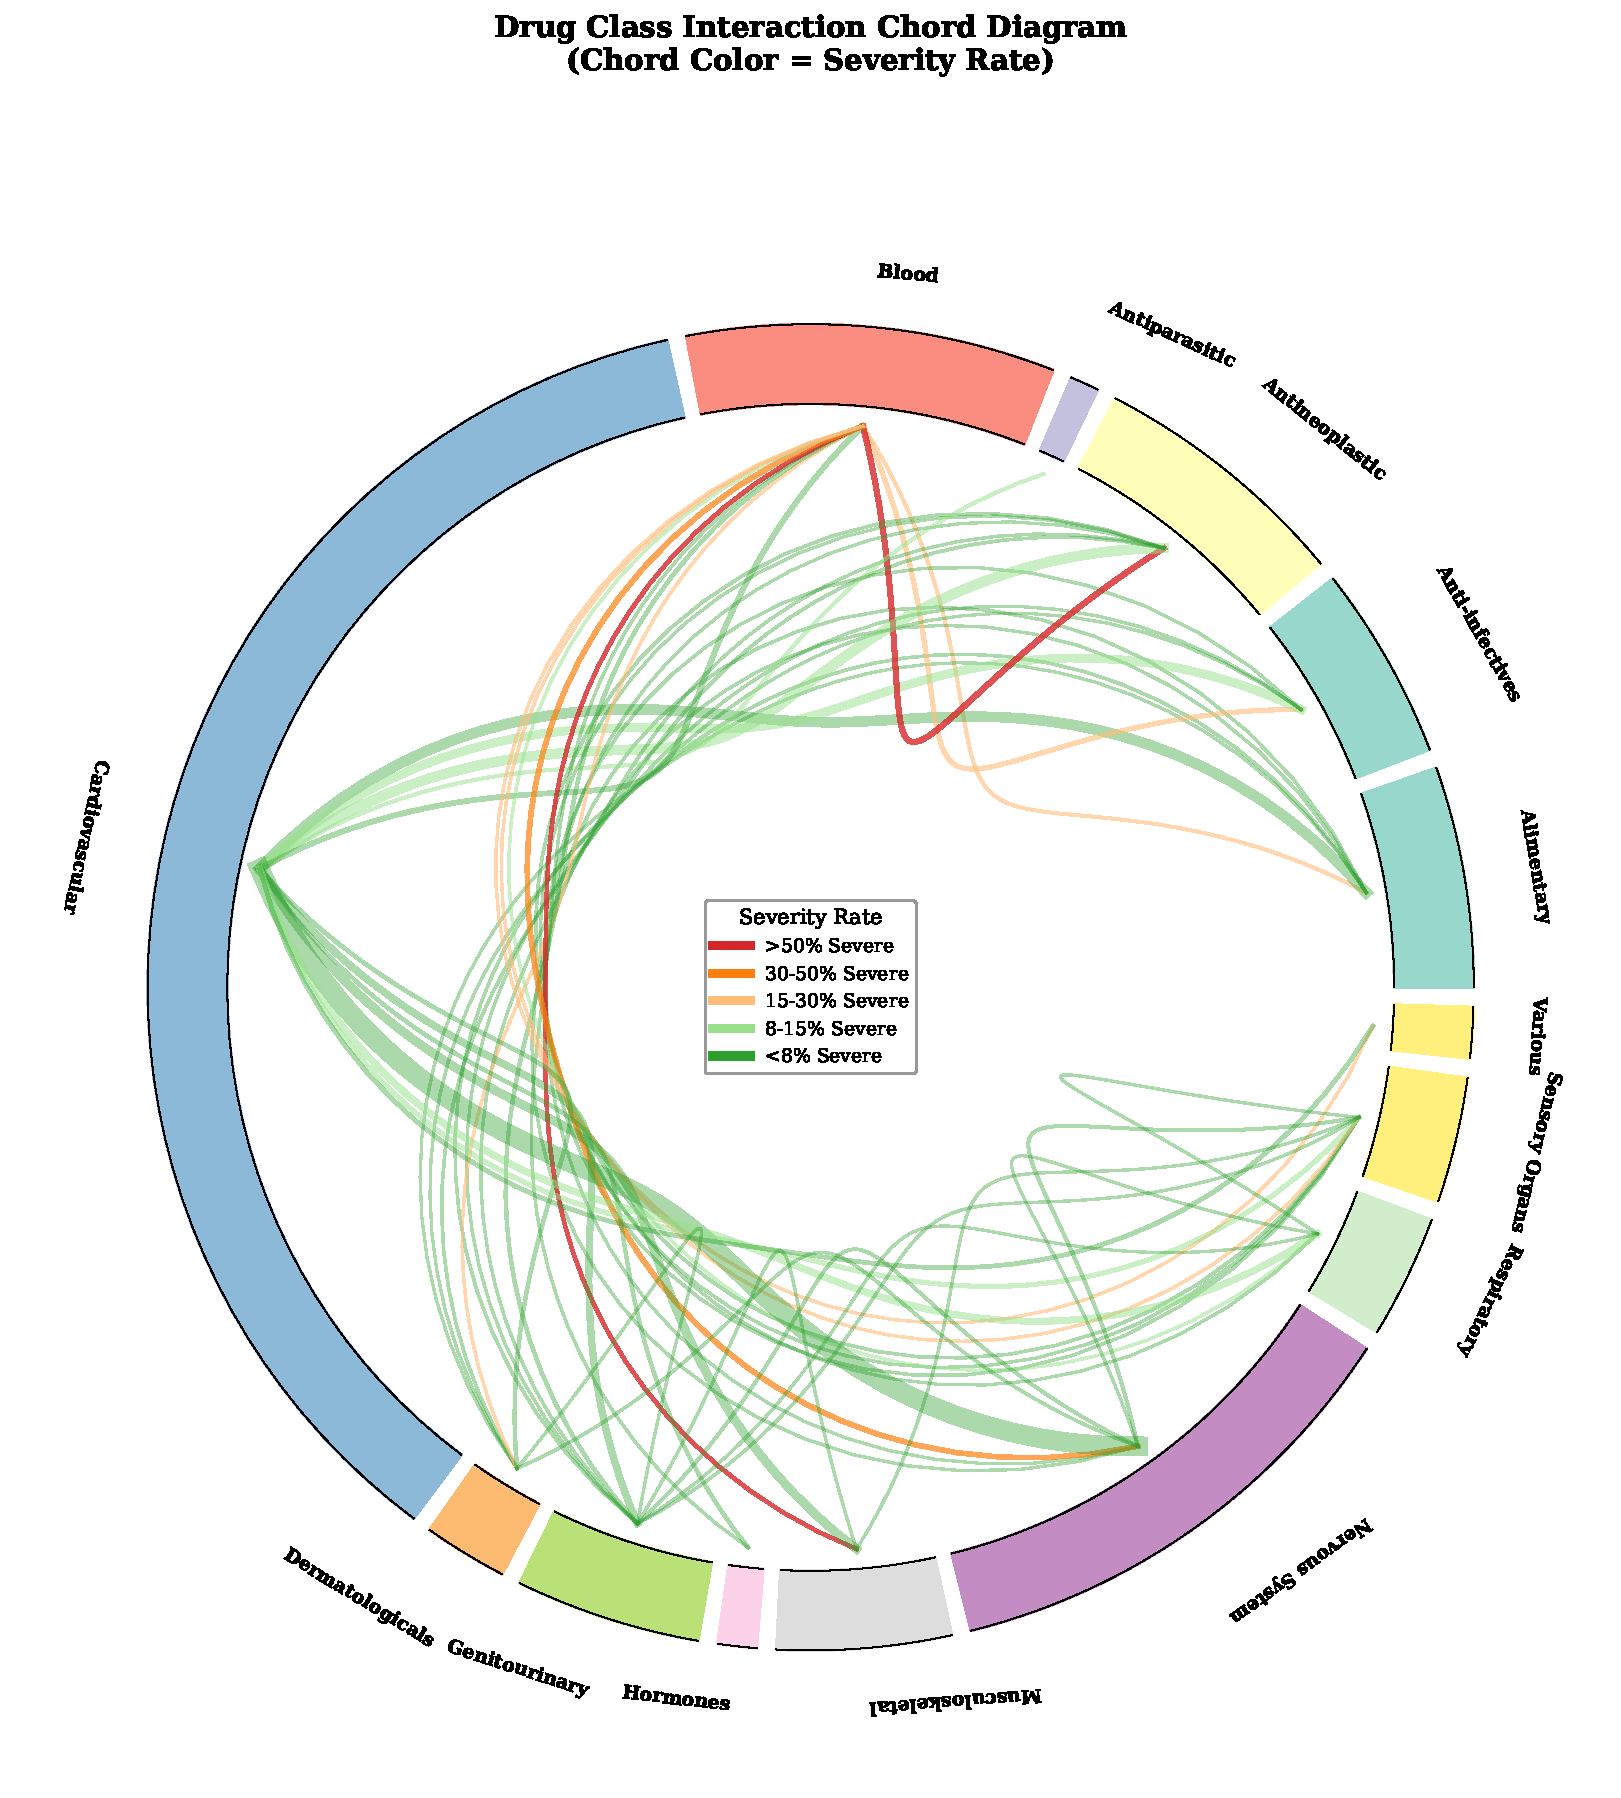
\includegraphics[width=0.8\textwidth]{figures/chord_severity.png}
\caption{Chord diagram visualizing drug-drug interactions by severity level. Arc width represents interaction volume between drug classes, with colors indicating severity: red for contraindicated, orange for major, yellow for moderate, and green for minor interactions.}
\label{fig:chord_severity}
\end{figure}

% Figure 2: Network Diagram with full names in legend
\begin{figure}[H]
\centering
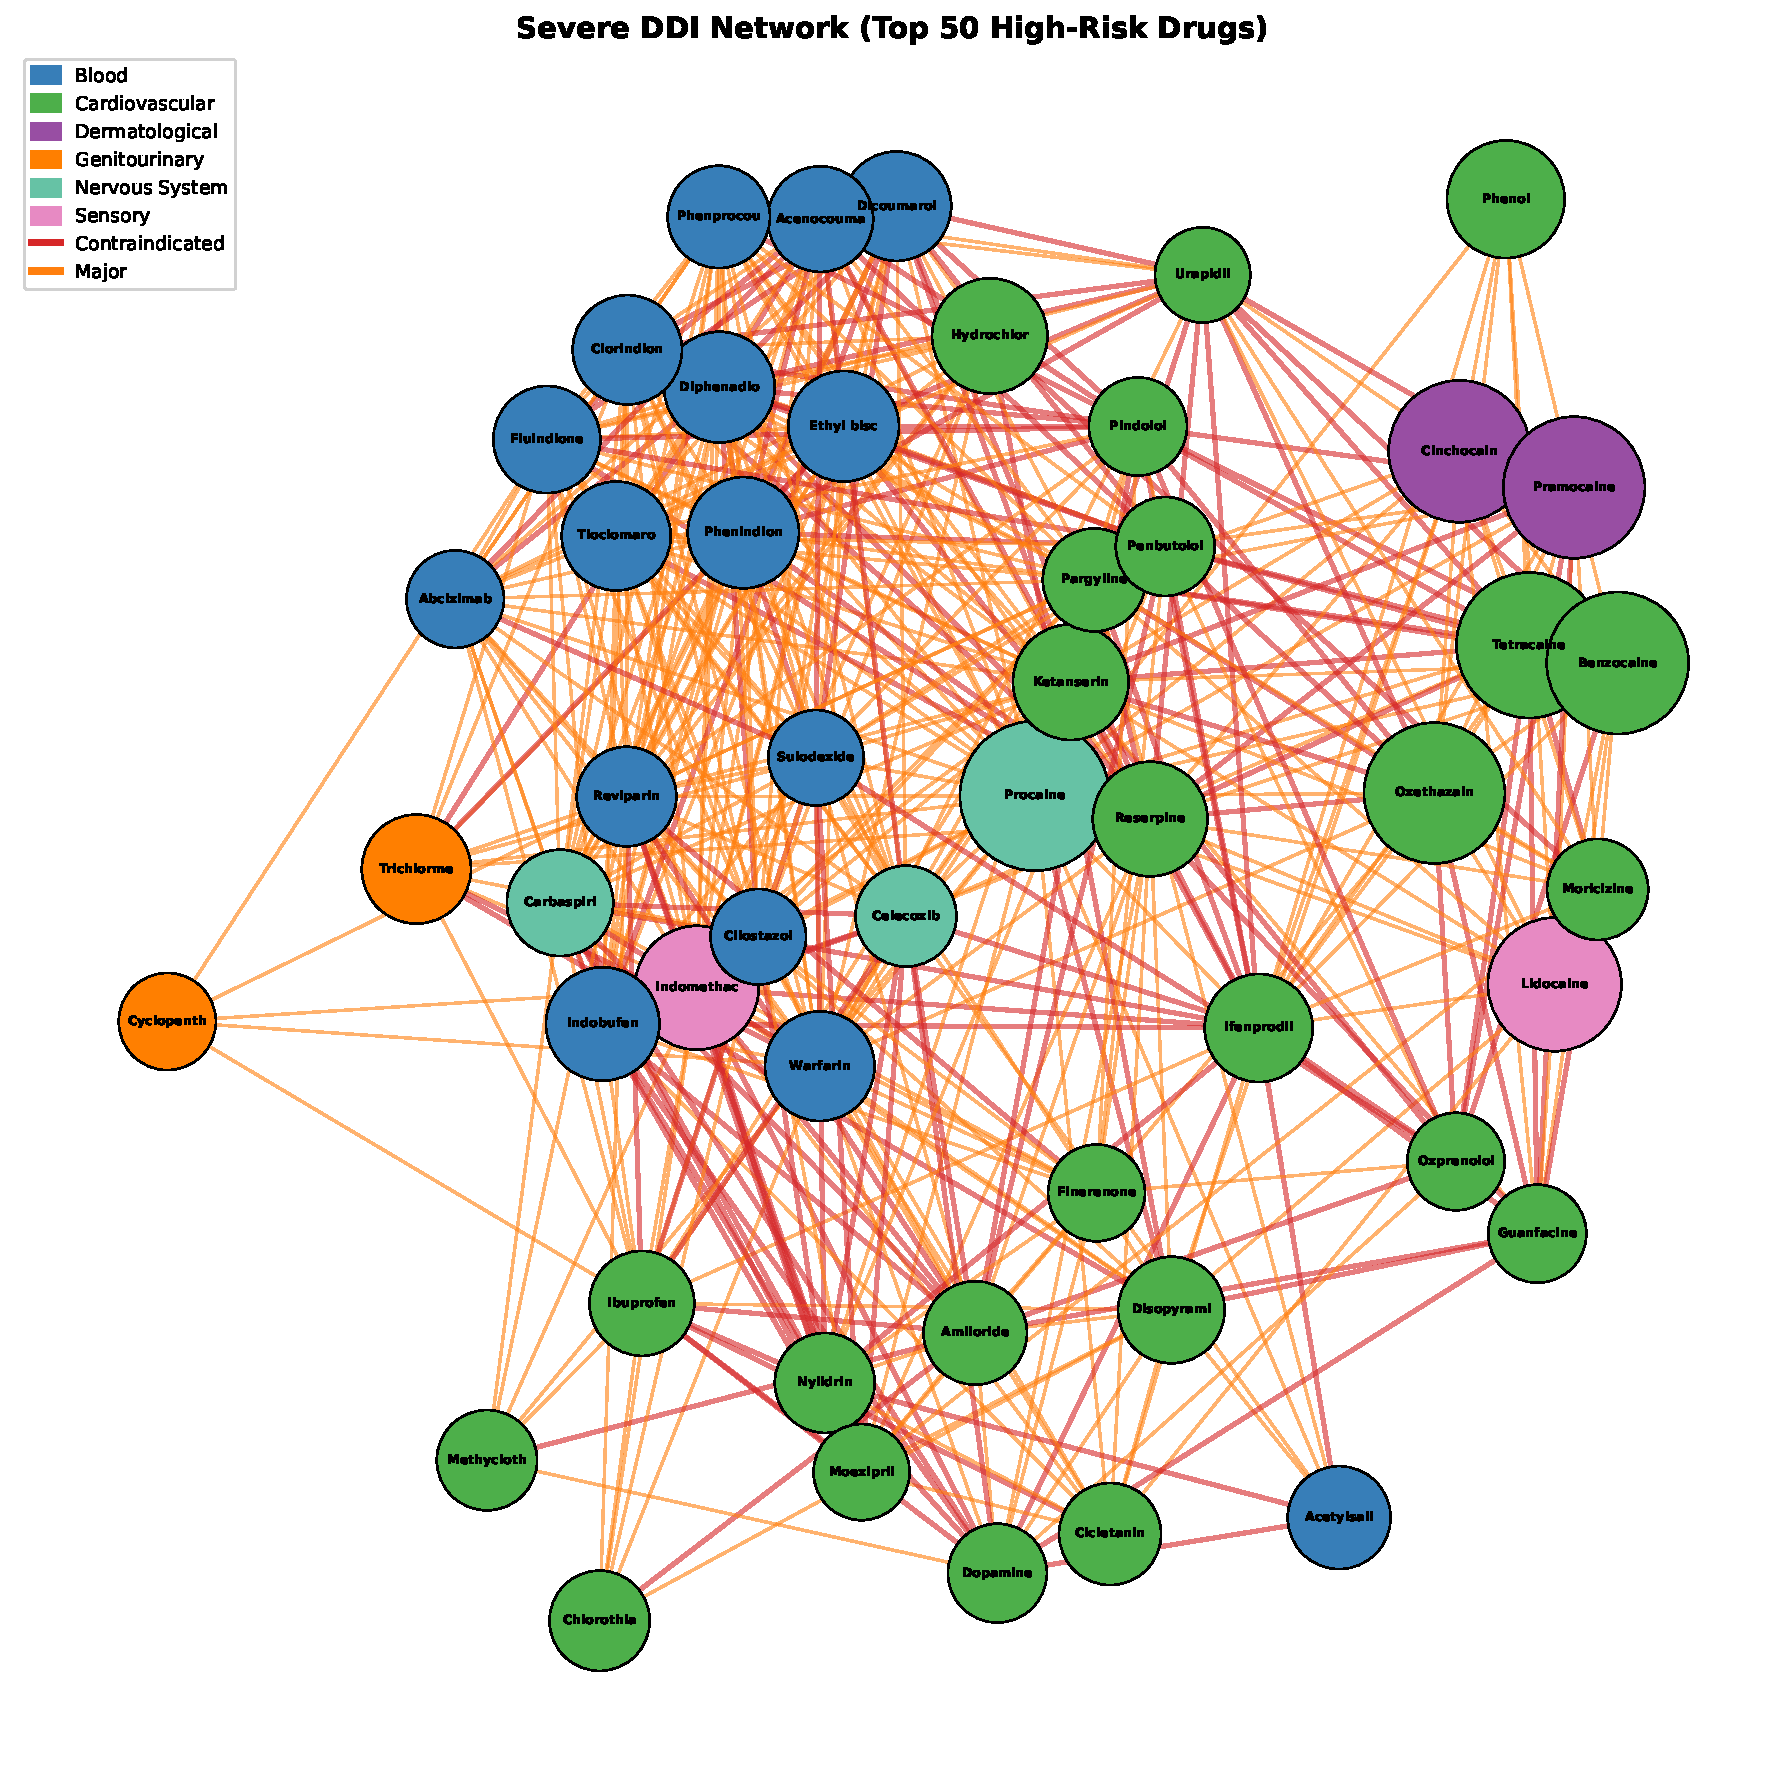
\includegraphics[width=0.9\textwidth]{figures/network_severe_ddi_compact.png}
\caption{Severe DDI network visualization showing the top 50 high-risk drugs. Node colors represent ATC drug classes (full names in legend), node size is proportional to severe interaction count. Edge colors encode severity: red = Contraindicated, orange = Major interactions.}
\label{fig:network_diagram}
\end{figure}

\subsection*{Polypharmacy Risk Index}

We developed the Polypharmacy Risk Index (PRI) to quantify individual drug risk within multi-drug regimens. The PRI combines four network-based metrics weighted according to their clinical relevance:

\begin{equation}
\text{PRI}(d) = 0.25 \cdot C_{\text{degree}}(d) + 0.30 \cdot C_{\text{weighted}}(d) + 0.20 \cdot C_{\text{betweenness}}(d) + 0.25 \cdot S(d)
\end{equation}

The degree centrality $C_{\text{degree}}(d)$ captures the interaction burden as the number of drugs interacting with drug $d$. The weighted degree $C_{\text{weighted}}(d)$ represents the severity-weighted sum of all interactions, giving greater importance to contraindicated and major interactions. Betweenness centrality $C_{\text{betweenness}}(d)$ quantifies the drug's role in risk propagation pathways across the network. The severity profile score $S(d)$ measures the proportion of a drug's interactions that are classified as contraindicated or major. Drugs with PRI scores exceeding 0.5 are classified as high-risk requiring immediate clinical review, scores between 0.3 and 0.5 indicate medium risk warranting close monitoring, and scores below 0.3 suggest lower risk with standard monitoring protocols.

\subsection*{Multi-Objective Drug Recommendation System}

The recommendation system employs a multi-objective optimization framework to identify therapeutic alternatives that balance clinical efficacy with safety. For each candidate alternative drug $d_{\text{alt}}$, we compute a recommendation score:

\begin{equation}
\text{RecScore}(d_{\text{alt}}) = 0.40 \cdot T(d_{\text{alt}}) + 0.35 \cdot SAF(d_{\text{alt}}) + 0.25 \cdot R(d_{\text{alt}})
\end{equation}

The therapeutic similarity score $T(d_{\text{alt}})$ (weight: 0.40) evaluates whether the alternative can serve the same clinical purpose as the original drug, incorporating ATC code matching for pharmacological class equivalence, shared protein targets indicating similar mechanisms of action, disease indication overlap confirming therapeutic applicability, and metabolic pathway similarity. The safety improvement score $SAF(d_{\text{alt}})$ (weight: 0.35) quantifies the reduction in DDI risk when the alternative is used with other drugs in the current regimen, penalizing contraindicated interactions heavily and major interactions moderately. The risk reduction score $R(d_{\text{alt}})$ (weight: 0.25) measures the net change in severe interactions (contraindicated plus major) and PRI score improvement.

\section*{Results}

\subsection*{Case Study: High-Risk Cardiovascular Polypharmacy}

We validated the methodology using a clinically realistic 5-drug cardiovascular regimen comprising Warfarin (anticoagulant), Amiodarone (antiarrhythmic), Digoxin (cardiac glycoside), Quinidine (antiarrhythmic), and Propranolol (beta-blocker). Analysis of this regimen against the DDI database revealed 10 severe drug-drug interactions: 2 contraindicated (Warfarin-Amiodarone causing increased bleeding risk, and Digoxin-Propranolol causing severe bradycardia) and 8 major interactions including combinations that increase drug concentrations, cause toxicity, or produce additive cardiac effects.

The multi-objective recommendation system identified Dabigatran (Direct Thrombin Inhibitor) as the optimal substitute for Warfarin with the highest recommendation score of 0.801. This score reflects strong performance across all three optimization objectives: therapeutic similarity of 0.850 indicating Dabigatran's suitability as an anticoagulant replacement, safety improvement of 0.782 reflecting minimal new DDI risks with the remaining drugs, and risk reduction of 0.750 representing substantial decrease in severe interactions. In comparison, other DOAC alternatives scored lower: Fondaparinux (0.524), Apixaban (0.385), Rivaroxaban (0.385), and Edoxaban (0.385).

Substituting Warfarin with Dabigatran reduced contraindicated interactions from 2 to 1 (50\% reduction), major interactions from 8 to 6 (25\% reduction), and total severe interactions from 10 to 7 (30\% reduction). The average PRI across the regimen decreased from 0.569 to 0.504, representing an 11.5\% improvement in the overall polypharmacy risk profile.

% Table 4: DOAC Alternatives Comparison
\begin{table}[H]
\centering
\caption{Multi-Objective Recommendation Scores for DOAC Alternatives}
\label{tab:doac_alternatives}
\begin{tabular}{@{}lcccccc@{}}
\toprule
\textbf{Drug} & \textbf{RecScore} & \textbf{Therap.} & \textbf{Safety} & \textbf{Risk$\downarrow$} & \textbf{Contra} & \textbf{Major} \\
\midrule
\textbf{Dabigatran} & \textbf{0.801} & 0.850 & 0.782 & 0.750 & 0 & 1 \\
Fondaparinux & 0.524 & 0.850 & 0.347 & 0.250 & 0 & 3 \\
Apixaban & 0.385 & 0.850 & 0.129 & 0.000 & 0 & 4 \\
Rivaroxaban & 0.385 & 0.850 & 0.129 & 0.000 & 0 & 4 \\
Edoxaban & 0.385 & 0.850 & 0.129 & 0.000 & 0 & 4 \\
\bottomrule
\end{tabular}
\end{table}

\subsection*{Network Visualization}

Figure~\ref{fig:polypharmacy_network} illustrates the before-and-after DDI network topology demonstrating how targeted drug substitution based on multi-objective recommendation scoring reduces network edge density and interaction severity. In the original network (left panel), Warfarin appears as a red node indicating its identification as the highest-risk drug, connected to other drugs through multiple contraindicated (red edges) and major (orange edges) interactions. Node sizes are proportional to PRI scores, visually indicating each drug's contribution to overall regimen risk.

The post-substitution network (right panel) shows Dabigatran as a green node representing the recommended substitute, with notably fewer and less severe connections to the remaining drugs. The reduction in red and orange edges directly corresponds to the elimination of one contraindicated and two major interactions. The recommendation score (0.801) displayed on the substitute drug node reflects the multi-objective optimization that balanced therapeutic equivalence with safety improvement and risk reduction.

\begin{figure}[h]
\centering
\includegraphics[width=\textwidth]{../polypharmacy_demo_output/03_before_after_comparison.png}
\caption{Polypharmacy DDI Network: Before and After Multi-Objective Recommendation-Based Drug Substitution. Left: Original high-risk regimen with Warfarin (red node) showing 2 contraindicated and 8 major interactions. Right: Optimized regimen after substituting Dabigatran (green node, Rec.Score = 0.801), reducing severe interactions by 30\%. Node size is proportional to PRI score. Edge colors encode severity: red = Contraindicated, orange = Major, yellow = Moderate.}
\label{fig:polypharmacy_network}
\end{figure}

% Data Sources Integration Figure
\begin{figure}[H]
\centering

\includegraphics[width=0.9\textwidth]{figures/fig4_data_sources.png}
\caption{Data source integration overview showing the contributions from DrugBank (primary DDI and drug metadata), SIDER (side effects), and CTD (disease associations) to the comprehensive knowledge graph.}
\label{fig:data_sources}
\end{figure}

% Severity Distribution Figure
\begin{figure}[H]
\centering

\includegraphics[width=0.8\textwidth]{figures/fig3_severity_distribution.png}
\caption{DDI severity distribution after recalibration using the empirical keyword-based classifier validated against DDInter database.}
\label{fig:severity_distribution}
\end{figure}

\section*{Conclusion}

The integration of network-based polypharmacy risk assessment with multi-objective drug recommendation provides a systematic framework for optimizing multi-drug regimens. By weighting therapeutic similarity (40\%), safety improvement (35\%), and risk reduction (25\%), the system identifies substitutes that maintain clinical efficacy while minimizing drug-drug interaction burden. The case study demonstrates a 30\% reduction in severe interactions through evidence-based drug substitution, supporting clinical decision-making in complex polypharmacy scenarios.

\section*{Data Availability}

The knowledge graph is available as a NetworkX pickle file with complete node and edge attributes, and as Neo4j-compatible CSV files for bulk import.

\bibliographystyle{plain}
\begin{thebibliography}{4}
\bibitem{wishart2018drugbank} Wishart DS, et al. DrugBank 5.0: a major update to the DrugBank database for 2018. \textit{Nucleic Acids Res}. 2018;46(D1):D1074-D1082.
\bibitem{kuhn2016sider} Kuhn M, et al. The SIDER database of drugs and side effects. \textit{Nucleic Acids Res}. 2016;44(D1):D1075-D1079.
\bibitem{davis2021ctd} Davis AP, et al. Comparative Toxicogenomics Database (CTD): update 2021. \textit{Nucleic Acids Res}. 2021;49(D1):D1138-D1143.
\bibitem{xiong2022ddinter} Xiong G, et al. DDInter: an online drug-drug interaction database. \textit{Nucleic Acids Res}. 2022;50(D1):D1200-D1207.
\end{thebibliography}

\end{document}
